\subsection{Diseño del barrido}

Se corrieron los ocho kernels de dataset GPU del catálogo bajo cinco
cadencias de muestreo NVML (1, 5, 10, 50 y 100\,ms), tres repeticiones cada
una (120 corridas reales). El valor de 100\,ms corresponde al \emph{default}
histórico del instrumento (\texttt{collector.hpp}), vigente en producción
hasta ARC-88 porque \texttt{gpu\_interval\_ns} nunca estuvo declarado como
campo real del manifiesto; 5\,ms es el valor adoptado en ese mismo cambio.

\subsection{El caso que motivó el cambio de producción}

\textbf{Nota sobre una corrección de datos}: la primera versión de este
barrido midió \texttt{rodinia\_heartwall} contra un video sintético que se había
corrompido silenciosamente a 25 cuadros (ver la Sección de hallazgos
colaterales del reporte extendido, ARC-89) -- la corrida fallaba de
inmediato pero seguía marcándose como exitosa, produciendo un patrón de
muestras artificialmente bajo que en un primer momento parecía ser el caso
más ajustado del barrido. Con el video corregido y el kernel re-medido,
\texttt{rodinia\_heartwall} deja de ser un caso límite en absoluto: el caso
real más ajustado es \texttt{rodinia\_backprop}.

La Figura~\ref{fig:gpu-interval} deja ver, con datos nuevos e
independientes de los usados durante la caracterización original, exactamente
el problema que ARC-83/84/86 ya habían diagnosticado con evidencia parcial:
a 100\,ms, \textbf{\texttt{rodinia\_backprop} logra apenas 9{,}0 muestras
NVML útiles en promedio}, apenas por encima del propio
\texttt{target\_windows\_per\_repetition=5}. A 5\,ms (el valor ahora
declarado en el manifiesto de producción), el mismo kernel logra 150{,}3
muestras: un salto de más de un orden de magnitud, no una mejora
incremental. \texttt{rodinia\_heartwall}, ya con datos correctos, se
comporta como el resto del catálogo (1063{,}7 muestras a 5\,ms, 60{,}3 a
100\,ms) -- nunca fue, en realidad, un caso cercano al límite.

\begin{figure}[H]
\centering
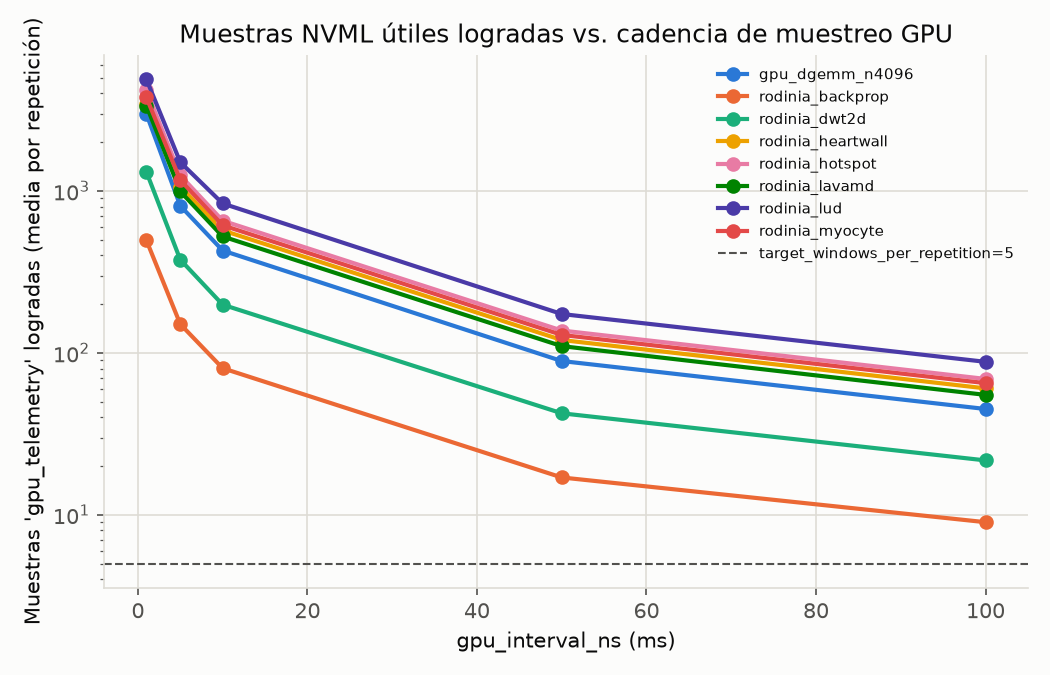
\includegraphics[width=0.85\textwidth]{../plots/gpu_interval_ns/gpu_telemetry_vs_interval.png}
\caption{Muestras NVML útiles logradas (media de 3 repeticiones) en
función de la cadencia de muestreo GPU, para los 8 kernels de dataset GPU
(datos corregidos). \texttt{rodinia\_backprop} es el caso más ajustado del
catálogo.}
\label{fig:gpu-interval}
\end{figure}

Los valores completos de \texttt{rodinia\_backprop} en las cinco cadencias
confirman que el descenso es monótono y suave, no un salto puntual:
150{,}3 muestras a 5\,ms, 80{,}3 a 10\,ms, 17{,}0 a 50\,ms, 9{,}0 a 100\,ms.
Es importante notar que 10\,ms \emph{también} supera el mínimo de 5 con
amplio margen ($16\times$). El valor correcto para describir 100\,ms, dado
el margen de solo $9/5=1{,}8\times$ sobre el mínimo configurado, no es
"insuficiente" en un sentido binario, sino \textbf{frágil y de muy baja
resolución temporal} -- técnicamente pasa el guardarraíl de
\texttt{target\_windows\_per\_repetition}, pero con un margen tan estrecho
que cualquier variación entre repeticiones podría hacerlo fallar. Este
barrido demuestra que 100\,ms es ese caso frágil y que 5\,ms (y también
10\,ms) son viables, pero no aísla a 5\,ms como el único valor correcto
frente a 10\,ms.

\subsection{Contar valores distintos no es lo mismo que contar actualizaciones del sensor}

Un supuesto implícito del argumento anterior es que cada lectura NVML
contada en la Figura~\ref{fig:gpu-interval} es una observación física
nueva. Se verificó esto inspeccionando los valores crudos de
\texttt{gpu\_power\_mw} y \texttt{gpu\_util\_pct} en \texttt{samples.csv}
para \texttt{rodinia\_backprop}, contando \textbf{cambios consecutivos de
valor} como indicador de una actualización real del sensor. Este método
tiene un límite metodológico que debe declararse: si dos actualizaciones
físicas consecutivas del sensor devuelven exactamente el mismo número
(plausible si la potencia se mantiene estable entre dos instantes), el
conteo de "valores distintos" las funde en una sola, subestimando el
número real de actualizaciones -- así que lo medido aquí es una \textbf{tasa
de refresco observada}, una cota inferior de la frecuencia real del
sensor, no una resolución física demostrada de forma directa.

Con esa salvedad, el patrón medido es de todas formas revelador: a 1\,ms
de cadencia (537 lecturas en 0{,}84\,s), solo se observan 7 valores
distintos de potencia, cada uno repetido en promedio 77 veces
consecutivas ($\approx$120\,ms de duración por escalón); a 5\,ms (151
lecturas), 8 valores distintos ($\approx$105\,ms por escalón); a 100\,ms
(9 lecturas), 7 valores distintos -- es decir, a 100\,ms el sondeo ya está
cerca de esta tasa de refresco observada, mientras que a 5\,ms la mayoría
de las "150 muestras" del argumento anterior comparten valor con su
vecina inmediata. \texttt{gpu\_util\_pct} exhibe el mismo patrón (3
valores distintos en 537 lecturas a 1\,ms). Esta periodicidad de
$\sim$105--120\,ms es, hasta donde se pudo verificar, un \textbf{hallazgo
empírico local de este nodo y esta GPU (A100)}: la documentación oficial
de NVML para \texttt{nvmlDeviceGetPowerUsage()} especifica que devuelve
potencia instantánea, pero no garantiza ni documenta una tasa de
actualización de 100--120\,ms -- no debe generalizarse a otro hardware sin
volver a medir.

Esto no invalida la elección de 5\,ms -- el número de lecturas de sondeo
\emph{sí} sigue siendo relevante para otras métricas que podrían variar
más rápido (temperatura, reloj SM, no verificadas aquí) y para reconstruir
la forma temporal de una transición de fase, y sondear más rápido que el
sensor nunca pierde información, solo genera redundancia -- pero sí obliga
a corregir el argumento cuantitativo: el margen "$30\times$" sobre el
objetivo de 5 ventanas cuenta en su mayoría redundancia del muestreo, no
información independiente nueva. La tasa de refresco \emph{observada} en
una corrida típica de \texttt{rodinia\_backprop} (0{,}84\,s) es de
aproximadamente 7--8 escalones distintos, ya cerca del límite de 5 -- un
margen mucho más ajustado que el que sugiere contar lecturas crudas,
aunque el número real de actualizaciones físicas podría ser algo mayor por
la limitación metodológica ya señalada.

\textbf{Conclusión (reformulada)}: la evidencia de este barrido respalda
adoptar 5\,ms como \textbf{valor viable y conservador, verificado en esta
plataforma}, y reclasificar 100\,ms de "insuficiente" a "frágil y de muy
baja resolución temporal, técnicamente por encima del mínimo configurado
pero sin margen real". No queda demostrado que 5\,ms sea el único punto
óptimo frente a 10\,ms (que también es viable y genera menos redundancia
de muestreo), ni que el margen efectivo sobre el mínimo de ventanas sea
tan amplio como sugiere el conteo ingenuo de lecturas -- ese margen real,
aproximado por la tasa de refresco observada y no por las lecturas de
sondeo, es sustancialmente más estrecho. Se recomienda, como extensión
concreta de este hallazgo, medir la duración de cada escalón y su
autocorrelación de forma más rigurosa (no solo contar valores distintos),
y verificar si otras métricas GPU usadas en el proyecto (reloj SM,
temperatura) comparten una tasa de refresco similar.
